% ============================================================
% fig_embeddings.tex — Espacio de embeddings
% Uso: % ============================================================
% fig_embeddings.tex — Espacio de embeddings
% Uso: % ============================================================
% fig_embeddings.tex — Espacio de embeddings
% Uso: % ============================================================
% fig_embeddings.tex — Espacio de embeddings
% Uso: \input{figures/fig_embeddings}
% ============================================================
\begin{figure}[H]
\centering

% --- Izquierda: representación one-hot ---
\begin{minipage}{0.35\textwidth}
\centering
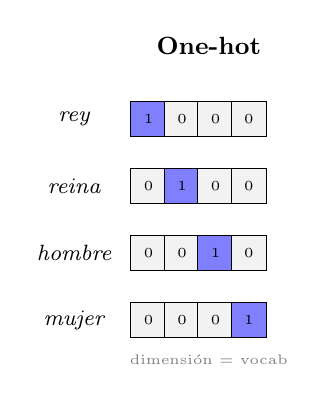
\begin{tikzpicture}[scale=0.85]

\node[font=\small\bfseries] at (1.5, 4.6) {One-hot};

% Vectores one-hot para 4 palabras
\foreach \word/\row/\col in {rey/0/0, reina/1/0, hombre/2/0, mujer/3/0}{
    \node[font=\footnotesize] at (-0.5, 3.5-\row) {\textit{\word}};
    \foreach \j in {0,1,2,3}{
        \pgfmathparse{int(\j==\row)}
        \ifnum\pgfmathresult=1
            \node[draw, fill=blue!50, minimum size=0.45cm, font=\tiny] at (0.6+\j*0.5, 3.5-\row) {1};
        \else
            \node[draw, fill=gray!10, minimum size=0.45cm, font=\tiny] at (0.6+\j*0.5, 3.5-\row) {0};
        \fi
    }
}
\node[font=\tiny, gray] at (1.5, -0.1) {dimensión = vocab};
\end{tikzpicture}
\end{minipage}
%
\hfill
%
% --- Flecha central ---
\begin{minipage}{0.08\textwidth}
\centering
\begin{tikzpicture}
\draw[-{Stealth}, very thick, blue!60] (0,1.8) -- (0.8,1.8);
\node[font=\tiny, blue!70, align=center] at (0.4, 2.2) {matriz\\$E$};
\end{tikzpicture}
\end{minipage}
%
\hfill
%
% --- Derecha: espacio de embeddings 2D ---
\begin{minipage}{0.50\textwidth}
\centering
\begin{tikzpicture}[scale=1.0]

\node[font=\small\bfseries] at (2.0, 4.3) {Espacio de embeddings};

\draw[-{Stealth}] (-0.2, 0) -- (4.2, 0) node[right, font=\tiny] {dim 1};
\draw[-{Stealth}] (0, -0.2) -- (0, 4.0) node[above, font=\tiny] {dim 2};

% Puntos
\fill[blue!70]       (1.0, 3.2) circle (4pt) node[above right, font=\footnotesize] {\textit{rey}};
\fill[purple!70]     (1.4, 3.6) circle (4pt) node[above right, font=\footnotesize] {\textit{reina}};
\fill[orange!80]     (1.0, 1.0) circle (4pt) node[below right, font=\footnotesize] {\textit{hombre}};
\fill[red!60]        (1.4, 1.4) circle (4pt) node[below right, font=\footnotesize] {\textit{mujer}};

% Vectores de analogía
\draw[dashed, blue!40]   (1.0,1.0) -- (1.0,3.2);
\draw[dashed, purple!40] (1.4,1.4) -- (1.4,3.6);
\draw[dashed, gray!50]   (1.0,3.2) -- (1.4,3.6);
\draw[dashed, gray!50]   (1.0,1.0) -- (1.4,1.4);

% Anotación analogía
\node[font=\tiny, gray, align=center] at (3.0, 2.3)
    {rey $-$ hombre\\$\approx$\\reina $-$ mujer};

\node[font=\tiny, gray] at (2.0, -0.5) {dimensión = $d_{\text{model}}$ (aprendida)};
\end{tikzpicture}
\end{minipage}

\caption{Comparación entre representación \textit{one-hot} (izquierda) y
espacio de \textit{embeddings} (derecha). La representación \textit{one-hot}
asigna un vector disperso a cada token sin capturar similitud semántica.
El \textit{embedding} proyecta cada token a un espacio denso de menor
dimensión donde las relaciones geométricas reflejan similitudes de
significado, como la conocida analogía \textit{rey} $-$ \textit{hombre}
$\approx$ \textit{reina} $-$ \textit{mujer}.}
\label{fig:embeddings}
\end{figure}

% ============================================================
\begin{figure}[H]
\centering

% --- Izquierda: representación one-hot ---
\begin{minipage}{0.35\textwidth}
\centering
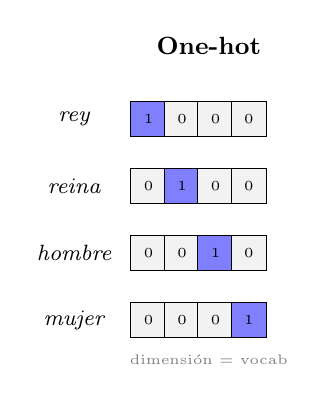
\begin{tikzpicture}[scale=0.85]

\node[font=\small\bfseries] at (1.5, 4.6) {One-hot};

% Vectores one-hot para 4 palabras
\foreach \word/\row/\col in {rey/0/0, reina/1/0, hombre/2/0, mujer/3/0}{
    \node[font=\footnotesize] at (-0.5, 3.5-\row) {\textit{\word}};
    \foreach \j in {0,1,2,3}{
        \pgfmathparse{int(\j==\row)}
        \ifnum\pgfmathresult=1
            \node[draw, fill=blue!50, minimum size=0.45cm, font=\tiny] at (0.6+\j*0.5, 3.5-\row) {1};
        \else
            \node[draw, fill=gray!10, minimum size=0.45cm, font=\tiny] at (0.6+\j*0.5, 3.5-\row) {0};
        \fi
    }
}
\node[font=\tiny, gray] at (1.5, -0.1) {dimensión = vocab};
\end{tikzpicture}
\end{minipage}
%
\hfill
%
% --- Flecha central ---
\begin{minipage}{0.08\textwidth}
\centering
\begin{tikzpicture}
\draw[-{Stealth}, very thick, blue!60] (0,1.8) -- (0.8,1.8);
\node[font=\tiny, blue!70, align=center] at (0.4, 2.2) {matriz\\$E$};
\end{tikzpicture}
\end{minipage}
%
\hfill
%
% --- Derecha: espacio de embeddings 2D ---
\begin{minipage}{0.50\textwidth}
\centering
\begin{tikzpicture}[scale=1.0]

\node[font=\small\bfseries] at (2.0, 4.3) {Espacio de embeddings};

\draw[-{Stealth}] (-0.2, 0) -- (4.2, 0) node[right, font=\tiny] {dim 1};
\draw[-{Stealth}] (0, -0.2) -- (0, 4.0) node[above, font=\tiny] {dim 2};

% Puntos
\fill[blue!70]       (1.0, 3.2) circle (4pt) node[above right, font=\footnotesize] {\textit{rey}};
\fill[purple!70]     (1.4, 3.6) circle (4pt) node[above right, font=\footnotesize] {\textit{reina}};
\fill[orange!80]     (1.0, 1.0) circle (4pt) node[below right, font=\footnotesize] {\textit{hombre}};
\fill[red!60]        (1.4, 1.4) circle (4pt) node[below right, font=\footnotesize] {\textit{mujer}};

% Vectores de analogía
\draw[dashed, blue!40]   (1.0,1.0) -- (1.0,3.2);
\draw[dashed, purple!40] (1.4,1.4) -- (1.4,3.6);
\draw[dashed, gray!50]   (1.0,3.2) -- (1.4,3.6);
\draw[dashed, gray!50]   (1.0,1.0) -- (1.4,1.4);

% Anotación analogía
\node[font=\tiny, gray, align=center] at (3.0, 2.3)
    {rey $-$ hombre\\$\approx$\\reina $-$ mujer};

\node[font=\tiny, gray] at (2.0, -0.5) {dimensión = $d_{\text{model}}$ (aprendida)};
\end{tikzpicture}
\end{minipage}

\caption{Comparación entre representación \textit{one-hot} (izquierda) y
espacio de \textit{embeddings} (derecha). La representación \textit{one-hot}
asigna un vector disperso a cada token sin capturar similitud semántica.
El \textit{embedding} proyecta cada token a un espacio denso de menor
dimensión donde las relaciones geométricas reflejan similitudes de
significado, como la conocida analogía \textit{rey} $-$ \textit{hombre}
$\approx$ \textit{reina} $-$ \textit{mujer}.}
\label{fig:embeddings}
\end{figure}

% ============================================================
\begin{figure}[H]
\centering

% --- Izquierda: representación one-hot ---
\begin{minipage}{0.35\textwidth}
\centering
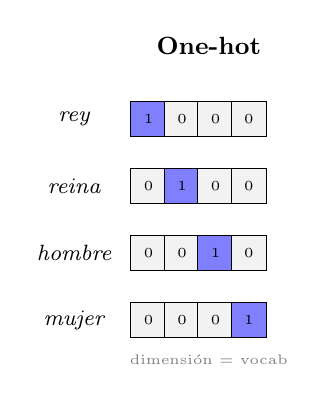
\begin{tikzpicture}[scale=0.85]

\node[font=\small\bfseries] at (1.5, 4.6) {One-hot};

% Vectores one-hot para 4 palabras
\foreach \word/\row/\col in {rey/0/0, reina/1/0, hombre/2/0, mujer/3/0}{
    \node[font=\footnotesize] at (-0.5, 3.5-\row) {\textit{\word}};
    \foreach \j in {0,1,2,3}{
        \pgfmathparse{int(\j==\row)}
        \ifnum\pgfmathresult=1
            \node[draw, fill=blue!50, minimum size=0.45cm, font=\tiny] at (0.6+\j*0.5, 3.5-\row) {1};
        \else
            \node[draw, fill=gray!10, minimum size=0.45cm, font=\tiny] at (0.6+\j*0.5, 3.5-\row) {0};
        \fi
    }
}
\node[font=\tiny, gray] at (1.5, -0.1) {dimensión = vocab};
\end{tikzpicture}
\end{minipage}
%
\hfill
%
% --- Flecha central ---
\begin{minipage}{0.08\textwidth}
\centering
\begin{tikzpicture}
\draw[-{Stealth}, very thick, blue!60] (0,1.8) -- (0.8,1.8);
\node[font=\tiny, blue!70, align=center] at (0.4, 2.2) {matriz\\$E$};
\end{tikzpicture}
\end{minipage}
%
\hfill
%
% --- Derecha: espacio de embeddings 2D ---
\begin{minipage}{0.50\textwidth}
\centering
\begin{tikzpicture}[scale=1.0]

\node[font=\small\bfseries] at (2.0, 4.3) {Espacio de embeddings};

\draw[-{Stealth}] (-0.2, 0) -- (4.2, 0) node[right, font=\tiny] {dim 1};
\draw[-{Stealth}] (0, -0.2) -- (0, 4.0) node[above, font=\tiny] {dim 2};

% Puntos
\fill[blue!70]       (1.0, 3.2) circle (4pt) node[above right, font=\footnotesize] {\textit{rey}};
\fill[purple!70]     (1.4, 3.6) circle (4pt) node[above right, font=\footnotesize] {\textit{reina}};
\fill[orange!80]     (1.0, 1.0) circle (4pt) node[below right, font=\footnotesize] {\textit{hombre}};
\fill[red!60]        (1.4, 1.4) circle (4pt) node[below right, font=\footnotesize] {\textit{mujer}};

% Vectores de analogía
\draw[dashed, blue!40]   (1.0,1.0) -- (1.0,3.2);
\draw[dashed, purple!40] (1.4,1.4) -- (1.4,3.6);
\draw[dashed, gray!50]   (1.0,3.2) -- (1.4,3.6);
\draw[dashed, gray!50]   (1.0,1.0) -- (1.4,1.4);

% Anotación analogía
\node[font=\tiny, gray, align=center] at (3.0, 2.3)
    {rey $-$ hombre\\$\approx$\\reina $-$ mujer};

\node[font=\tiny, gray] at (2.0, -0.5) {dimensión = $d_{\text{model}}$ (aprendida)};
\end{tikzpicture}
\end{minipage}

\caption{Comparación entre representación \textit{one-hot} (izquierda) y
espacio de \textit{embeddings} (derecha). La representación \textit{one-hot}
asigna un vector disperso a cada token sin capturar similitud semántica.
El \textit{embedding} proyecta cada token a un espacio denso de menor
dimensión donde las relaciones geométricas reflejan similitudes de
significado, como la conocida analogía \textit{rey} $-$ \textit{hombre}
$\approx$ \textit{reina} $-$ \textit{mujer}.}
\label{fig:embeddings}
\end{figure}

% ============================================================
\begin{figure}[H]
\centering

% --- Izquierda: representación one-hot ---
\begin{minipage}{0.35\textwidth}
\centering
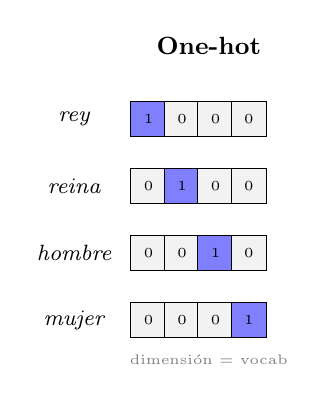
\begin{tikzpicture}[scale=0.85]

\node[font=\small\bfseries] at (1.5, 4.6) {One-hot};

% Vectores one-hot para 4 palabras
\foreach \word/\row/\col in {rey/0/0, reina/1/0, hombre/2/0, mujer/3/0}{
    \node[font=\footnotesize] at (-0.5, 3.5-\row) {\textit{\word}};
    \foreach \j in {0,1,2,3}{
        \pgfmathparse{int(\j==\row)}
        \ifnum\pgfmathresult=1
            \node[draw, fill=blue!50, minimum size=0.45cm, font=\tiny] at (0.6+\j*0.5, 3.5-\row) {1};
        \else
            \node[draw, fill=gray!10, minimum size=0.45cm, font=\tiny] at (0.6+\j*0.5, 3.5-\row) {0};
        \fi
    }
}
\node[font=\tiny, gray] at (1.5, -0.1) {dimensión = vocab};
\end{tikzpicture}
\end{minipage}
%
\hfill
%
% --- Flecha central ---
\begin{minipage}{0.08\textwidth}
\centering
\begin{tikzpicture}
\draw[-{Stealth}, very thick, blue!60] (0,1.8) -- (0.8,1.8);
\node[font=\tiny, blue!70, align=center] at (0.4, 2.2) {matriz\\$E$};
\end{tikzpicture}
\end{minipage}
%
\hfill
%
% --- Derecha: espacio de embeddings 2D ---
\begin{minipage}{0.50\textwidth}
\centering
\begin{tikzpicture}[scale=1.0]

\node[font=\small\bfseries] at (2.0, 4.3) {Espacio de embeddings};

\draw[-{Stealth}] (-0.2, 0) -- (4.2, 0) node[right, font=\tiny] {dim 1};
\draw[-{Stealth}] (0, -0.2) -- (0, 4.0) node[above, font=\tiny] {dim 2};

% Puntos
\fill[blue!70]       (1.0, 3.2) circle (4pt) node[above right, font=\footnotesize] {\textit{rey}};
\fill[purple!70]     (1.4, 3.6) circle (4pt) node[above right, font=\footnotesize] {\textit{reina}};
\fill[orange!80]     (1.0, 1.0) circle (4pt) node[below right, font=\footnotesize] {\textit{hombre}};
\fill[red!60]        (1.4, 1.4) circle (4pt) node[below right, font=\footnotesize] {\textit{mujer}};

% Vectores de analogía
\draw[dashed, blue!40]   (1.0,1.0) -- (1.0,3.2);
\draw[dashed, purple!40] (1.4,1.4) -- (1.4,3.6);
\draw[dashed, gray!50]   (1.0,3.2) -- (1.4,3.6);
\draw[dashed, gray!50]   (1.0,1.0) -- (1.4,1.4);

% Anotación analogía
\node[font=\tiny, gray, align=center] at (3.0, 2.3)
    {rey $-$ hombre\\$\approx$\\reina $-$ mujer};

\node[font=\tiny, gray] at (2.0, -0.5) {dimensión = $d_{\text{model}}$ (aprendida)};
\end{tikzpicture}
\end{minipage}

\caption{Comparación entre representación \textit{one-hot} (izquierda) y
espacio de \textit{embeddings} (derecha). La representación \textit{one-hot}
asigna un vector disperso a cada token sin capturar similitud semántica.
El \textit{embedding} proyecta cada token a un espacio denso de menor
dimensión donde las relaciones geométricas reflejan similitudes de
significado, como la conocida analogía \textit{rey} $-$ \textit{hombre}
$\approx$ \textit{reina} $-$ \textit{mujer}.}
\label{fig:embeddings}
\end{figure}
